\documentclass[tikz]{standalone}
    \usepackage{tikz}
    \usetikzlibrary{positioning, graphs}
    \usetikzlibrary{graphs.standard}
    \begin{document}
    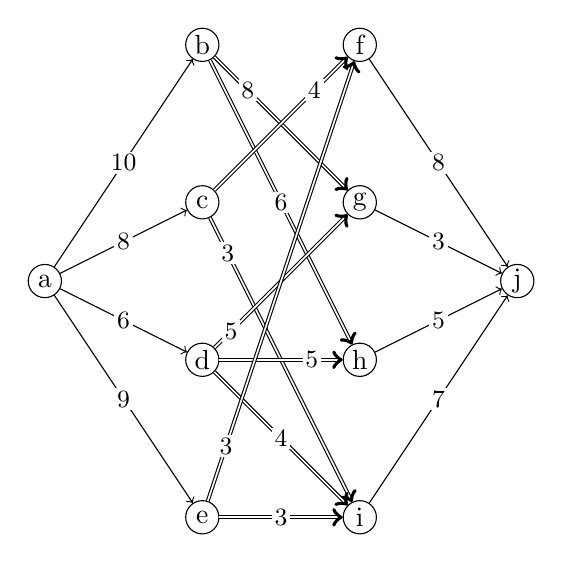
\begin{tikzpicture}
    \begin{scope}
            [vertex/.style={draw,circle,inner sep = 0em, minimum size = 1.2em},
             edgelabel/.style = {fill = white, inner sep = 0.1em, font=\small}]
            \node[vertex] (a) at (0,0) {a};
            \node[vertex] (b) at (2,3) {b};
            \node[vertex] (c) at (2,1) {c};
            \node[vertex] (d) at (2,-1) {d};
            \node[vertex] (e) at (2,-3) {e};
            \node[vertex] (f) at (4,3) {f};
            \node[vertex] (g) at (4,1) {g};
            \node[vertex] (h) at (4,-1) {h};
            \node[vertex] (i) at (4,-3) {i};
            \node[vertex] (j) at (6,0) {j};
            
            \draw[->] (a) to node[edgelabel] {$10$} (b);
            \draw[->] (a) to node[edgelabel] {$8$} (c);
            \draw[->] (a) to node[edgelabel] {$6$} (d);
            \draw[->] (a) to node[edgelabel] {$9$} (e);
            \draw[->, double] (b) to node[edgelabel, near start] {$8$} (g);
            \draw[->, double] (b) to node[edgelabel] {$6$} (h);
            \draw[->, double] (c) to node[edgelabel, near end] {$4$} (f);
            \draw[->, double] (c) to node[edgelabel, very near start] {$3$} (i);
            \draw[->, double] (d) to node[edgelabel, very near start] {$5$} (g);
            \draw[->, double] (d) to node[edgelabel, near end] {$5$} (h);
            \draw[->, double] (d) to node[edgelabel] {$4$} (i);
            \draw[->, double] (e) to node[edgelabel, very near start] {$3$} (f);
            \draw[->, double] (e) to node[edgelabel] {$3$} (i);
            \draw[->] (f) to node[edgelabel] {$8$} (j);
            \draw[->] (g) to node[edgelabel] {$3$} (j);
            \draw[->] (h) to node[edgelabel] {$5$} (j);
            \draw[->] (i) to node[edgelabel] {$7$} (j);
    \end{scope}
    \end{tikzpicture}
    \end{document}